\documentclass[11pt,letterpaper]{article}
\usepackage[lmargin=1in,rmargin=1in,tmargin=1in,bmargin=1in]{geometry}
\usepackage{../style/homework}
\usepackage{../style/commands}
\setbool{quotetype}{true} % True: Side; False: Under
\setbool{hideans}{false} % Student: True; Instructor: False

% -------------------
% Content
% -------------------
\begin{document}

\homework{8: Due 10/17}{The consequences of an act affect the probability of its occurring again.}{B.F. Skinner}

% Problem 1
\problem{10} The probabilities of several events in a finite probability space are given below:
	\[
	\begin{aligned}
	P(A)&= 0.45 &\qquad\qquad P(D)&= 0.10 \\
	P(B)&= 0.20 & P(A \text{ and } C)&= 0.01 \\
	P(C)&= 0.85 & P(B \text{ and } C)&= 0.10 
	\end{aligned}
	\] 
\begin{enumerate}[(a)]
\item Assuming that $A$ and $B$ are independent, find $P(A \text{ or } B)$.
\item Assuming $C$ and $D$ are disjoint, find $P(C \text{ or } D)$.
\item Are $B$ and $C$ disjoint? Explain.
\item Are $A$ and $C$ independent? Explain. 
\item Find $P(B \;|\; C)$.
\end{enumerate} \pspace

\sol 
\begin{enumerate}[(a)]
\item We know that $P(A \text{ or } B)= P(A) + P(B) - P(A \text{ and } B)$. If $A, B$ are independent, then $P(A \text{ and } B)= P(A) P(B)$. But then $P(A \text{ and } B)= P(A) P(B)= 0.45 \cdot 0.20= 0.09$. But then\dots
	\[
	P(A \text{ or } B)= P(A) + P(B) - P(A \text{ and } B)= 0.45 + 0.20 - 0.09= 0.56
	\] \pspace

\item Because $C$ and $D$ are disjoint, $P(C \text{ and } D)= 0$. But then\dots
	\[
	P(C \text{ or } D)= P(C) + P(D) - P(C \text{ and } D)= 0.85 + 0.10 - 0= 0.95
	\]
Generally, if events $E$ and $F$ are disjoint, $P(E \text{ or } F)= P(E) + P(F)$. \pspace

\item If $B$ and $C$ were disjoint, then $P(B \text{ or } C)= P(B) + P(C)$. But then $P(B \text{ or } C)= 0.20 + 0.85= 1.05 > 1$, which is impossible. Therefore, $B$ and $C$ cannot be disjoint. \pspace

\item If $A$ and $C$ were independent, then $P(A \text{ and } C)= P(A) P(C)$. But then $P(A \text{ and } C)= 0.01 \neq 0.3825= 0.45 \cdot 0.85= P(A) P(C)$. Therefore, $A$ and $C$ are not independent. \pspace

\item We know that\dots
	\[
	P(B \;|\; C)= \dfrac{P(B \text{ and } C)}{P(B)}= \dfrac{0.10}{0.20}= 0.50
	\]
\end{enumerate}



\newpage



% Problem 2
\problem{10} A statistician is examining tax rebates for small businesses in the area. She finds that of the 227 small businesses in the county, 109 qualified for a state tax rebate, 80 qualified for a federal tax rebate, and 38 qualified for both. 
	\begin{enumerate}[(a)]
	\item Find the probability that a randomly selected local small business qualified for a state or federal tax rebate. 
	\item Find the probability that a randomly selected local small business qualified for a state and federal tax rebate. 
	\item Find the probability that a randomly selected local small business qualified for neither a state nor a federal tax rebate. 
	\item Find the probability that a randomly selected local small business qualified for only a state tax rebate. 
	\item Find the probability that a randomly selected local small business that qualified for a state tax rebate also qualified for a federal tax rebate. 
	\end{enumerate} \pspace

\sol 
\begin{enumerate}[(a)]
\item 
	\[
	\hspace{-1.75cm} P(\text{State or Federal})= P(\text{State}) + P(\text{Federal}) - P(\text{State \& Federal})= \dfrac{109}{227} + \dfrac{80}{227} - \dfrac{38}{227}= \dfrac{71 + 38 + 42}{227}= \dfrac{151}{227} \approx 0.6652
	\] \pspace

\item 
	\[
	P(\text{State and Federal})= \dfrac{38}{227} \approx 0.1674
	\] \pspace

\item 
	\[
	P(\text{Neither State nor Federal})= 1 - P(\text{State or Federal})= 1 - \dfrac{151}{227}= \dfrac{76}{227} \approx 0.3363
	\] \pspace

\item 
	\[
	P(\text{Only State})= P(\text{State}) - P(\text{State \& Federal})= \dfrac{109}{227} - \dfrac{38}{227}= \dfrac{42}{227} \approx 0.1850
	\] \pspace

\item 
	\[
	P(\text{Federal} \;|\; \text{State})= \dfrac{P(\text{Federal \& State})}{P(\text{State})}= \dfrac{38/227}{109/227}= \dfrac{38}{109} \approx 0.3486
	\]
\end{enumerate}

	\vfill
	
	\[
	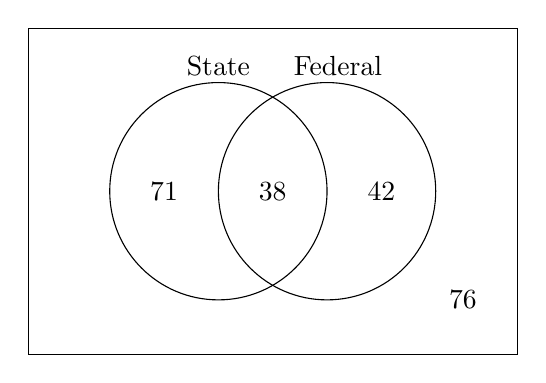
\begin{tikzpicture}[scale=0.69]
	\draw (0,0) rectangle (9,6);
	\draw (3.5,3) circle (2);
	\draw (5.5,3) circle (2);
	
	\node at (3.5,5.3) {State};
	\node at (5.7,5.3) {Federal}; 
	
	\node at (2.5,3) {71};
	\node at (4.5,3) {38};
	\node at (6.5,3) {42};
	\node at (8,1) {76};
	\end{tikzpicture}
	\]



\newpage



% Problem 2
\problem{10} A large accounting class has 156 students. A chart summarizing the pass/fail/withdraw results for students, broken down by class, is given below. \par
	\begin{table}[H]
	\centering
	\begin{tabular}{lccc}
	& Pass & Fail & Withdraw \\ \cline{2-4} 
	\multicolumn{1}{l|}{Freshmen} & \multicolumn{1}{c|}{41} & \multicolumn{1}{c|}{14} & \multicolumn{1}{c|}{6} \\ \cline{2-4} 
	\multicolumn{1}{l|}{Sophomore} & \multicolumn{1}{c|}{56} & \multicolumn{1}{c|}{11} & \multicolumn{1}{c|}{3} \\ \cline{2-4} 
	\multicolumn{1}{l|}{Junior} & \multicolumn{1}{c|}{18} & \multicolumn{1}{c|}{3} & \multicolumn{1}{c|}{1} \\ \cline{2-4} 
	\multicolumn{1}{l|}{Senior} & \multicolumn{1}{c|}{3} & \multicolumn{1}{c|}{0} & \multicolumn{1}{c|}{0} \\ \cline{2-4} 
	\end{tabular}
	\end{table} \pspace
Given the data above, answer the following:
	\begin{enumerate}[(a)]
	\item Find the probability that a randomly selected student failed the course.
	\item Find the probability that a randomly selected student was a sophomore or withdrew from the course.
	\item Find the probability that a randomly selected student was a junior and failed the course.
	\item Find the probability that a randomly selected freshman failed the course.
	\item Are freshmen status and failing the course independent events? Explain. 
	\end{enumerate} \pspace

\sol First, we should find the totals for each row/column:
	\begin{table}[H]
	\centering
	\begin{tabular}{lcccc}
	& Pass & Fail & Withdraw & {\itshape Total} \\ \cline{2-4} 
	\multicolumn{1}{l|}{Freshmen} & \multicolumn{1}{c|}{41} & \multicolumn{1}{c|}{14} & \multicolumn{1}{c|}{6} & 61 \\ \cline{2-4} 
	\multicolumn{1}{l|}{Sophomore} & \multicolumn{1}{c|}{56} & \multicolumn{1}{c|}{11} & \multicolumn{1}{c|}{3} & 70 \\ \cline{2-4} 
	\multicolumn{1}{l|}{Junior} & \multicolumn{1}{c|}{18} & \multicolumn{1}{c|}{3} & \multicolumn{1}{c|}{1} & 22 \\ \cline{2-4} 
	\multicolumn{1}{l|}{Senior} & \multicolumn{1}{c|}{3} & \multicolumn{1}{c|}{0} & \multicolumn{1}{c|}{0} & 3 \\ \cline{2-4}
	{\itshape Total} & 118 & 28 & 10 & 156
	\end{tabular}
	\end{table}

\begin{enumerate}[(a)]
\item 
	\[
	P(\text{failed})= \dfrac{28}{156}= \dfrac{7}{39} \approx 0.1795
	\]

\item 
	\[
	P(\text{soph or withd})= \dfrac{70 + 10 - 3}{156}= \dfrac{77}{156} \approx 0.4936
	\]

\item 
	\[
	P(\text{junior and fail})= \dfrac{3}{156}= \dfrac{1}{52} \approx 0.0192
	\]

\item 
	\[
	P(\text{fail} \;|\; \text{fresh})= \dfrac{P(\text{fail and fresh})}{P(\text{fresh})}= \dfrac{14}{61} \approx 0.2295
	\]

\item If they were independent, then $P(\text{fresh and fail})= P(\text{fresh}) P(\text{fail})$. But $P(\text{fresh and fail})= \frac{14}{156}= 0.0897 \neq 0.0702= \frac{61}{156} \cdot \frac{28}{156}= P(\text{fresh}) P(\text{fail})$. Therefore, they are not independent. Alternatively, if they were independent, then $P(\text{fail} \;|\; \text{fresh})= P(\text{fail})$. But by (a) and (d), $P(\text{fail} \;|\; \text{fresh})= 0.2295 \neq 0.1795= P(\text{fail})$.
\end{enumerate}



\newpage



% Problem 4
\problem{10} Administrators at a college are examining job placement for their graduates. Only 4\% of their graduates are Computer Science majors. They find that 85\% of their computer science majors obtain a job within 6~months of graduating. For all other majors at the college, 70\% of their graduates find a job within 6~months of graduating. 
	\begin{enumerate}[(a)]
	\item Find the percentage of graduates that received a job within 6~months of graduating. 
	\item Find the percentage of graduates that were a computer science major and obtained a job within 6~months of graduating.
	\item Find the percentage of graduates that obtained a job within 6~months of graduating or were not a computer science major. 
	\item Of the graduates that obtained a job within 6~months of graduating, what percentage were computer science majors?	
	\end{enumerate} \pspace

\sol 
\begin{enumerate}[(a)]
\item 
	\[
	P(\text{Job})= 0.0340 + 0.6720= 0.7060
	\] \pspace

\item 
	\[
	P(\text{CS \& Job})= 0.0340
	\] \pspace

\item 
	\[
	P(\text{Job or Not CS})= 0.0340 + 0.6720 + 0.2880= 0.994
	\] \pspace

\item 
	\[
	P(\text{CS})= 0.0340 + 0.0060= 0.04
	\]
\end{enumerate} \pspace

		\[
		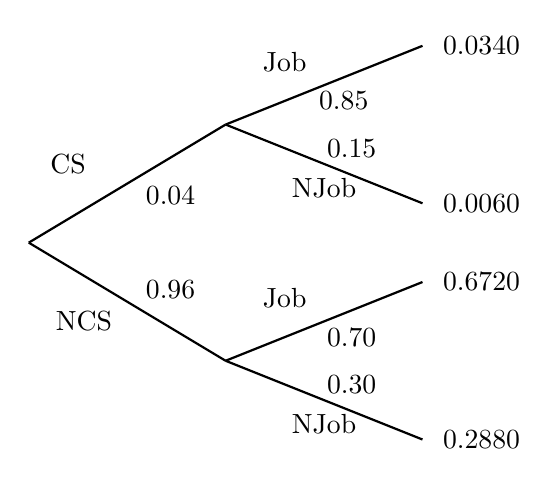
\begin{tikzpicture}[scale= 1.0]
		\def\FirstUpLabel{CS}
		\def\FirstDownLabel{NCS}
		\def\SecondUpLabel{Job}
		\def\SecondDownLabel{NJob}
		\def\Up{$0.04$}
		\def\Down{$0.96$}
		\def\UpUp{$0.85$}
		\def\UpDown{$0.15$}
		\def\DownUp{$0.70$}
		\def\DownDown{$0.30$}
		\def\first{$0.0340$}
		\def\second{$0.0060$}
		\def\third{$0.6720$}
		\def\fourth{$0.2880$}
		
		\node at (0.5,1) {\FirstUpLabel};	
		\node at (0.7,-1) {\FirstDownLabel};	
		\node at (1.8,0.6) {\Up};
		\node at (1.8,-0.6) {\Down};
		\draw[thick] (0,0) -- (2.5,1.5);
		\draw[thick] (0,0) -- (2.5,-1.5);
		
		\node at (3.25,2.3) {\SecondUpLabel};
		\node at (3.75,0.7) {\SecondDownLabel};
		\node at (4,1.8) {\UpUp};
		\node at (4.1,1.2) {\UpDown};
		\node at (5.75,2.5) {\first};
		\node at (5.75,0.5) {\second};
		\draw[thick] (2.5,1.5) -- (5,2.5);
		\draw[thick] (2.5,1.5) -- (5,0.5);

		\node at (3.25,-0.7) {\SecondUpLabel};
		\node at (3.75,-2.3) {\SecondDownLabel};
		\node at (4.1,-1.2) {\DownUp};
		\node at (4.1,-1.8) {\DownDown};
		\node at (5.75,-0.5) {\third};	
		\node at (5.75,-2.5) {\fourth};	
		\draw[thick] (2.5,-1.5) -- (5,-0.5);
		\draw[thick] (2.5,-1.5) -- (5,-2.5);
		\end{tikzpicture}
		\]


\end{document}